
\begin{center}
	{\scriptsize
		\begin{tabularx}{\textwidth}{p{0.2\textwidth}|p{0.6\textwidth}|p{0.1\textwidth}}
			\caption{Summary of methods for achieving the objectives} \label{tab:achieve_objective} \\
			\hline 
			\hline 
			\textbf{Objectives} & 
			\textbf{Methods} & 
			\textbf{Locations} \\ 
			\hline 
			\endfirsthead
			\multicolumn{3}{c}%
			{\textit{Continued from previous page}} \\
			\hline
			\hline 
			\textbf{Objectives} & 
			\textbf{Methods} & 
			\textbf{Locations} \\ 
			\hline 
			\endhead
			\hline 
			\multicolumn{3}{r}{\textit{Continued on next page}} \\ 
			\endfoot
			\hline 
			\endlastfoot
			\hline
			
			\Paste{GO} & 
			Results:
			\begin{enumerate}
				\item Successfully developed a user-priority-based grading and sorting system using machine learning and computer vision which can assess the mangoes’ ripeness, size and bruises.
			\end{enumerate} 
			% Actual Results:
			% \begin{enumerate}
			% 	\item More work needs to be done to fine tune the software components to achieve higher accuracy such as changing hyperparameters or using a newer version of EfficientNet
			% 	\item More work needs to be done to make the hardware component more robust such as by fixing the camera and LED lights in place
			% \end{enumerate} 
			& Sec.~\ref{sec:summary_results_and_discussions} on p.~\pageref{sec:summary_results_and_discussions} \\ \hline
			
			\Paste{SO1} & 
			Results:
			\begin{enumerate}
				\item Successfully integrated a conveyor belt with the image acquisition in order to achieve efficient flow of automated sorting and grading of the mangoes.  
				\item Successfully integrated LED strips to provide optimal lighting for image capturing of the mangoes.
				\item Successfully fixed the hardware components in place
			\end{enumerate} 
			% Actual Results:
			% \begin{enumerate}
			% 	\item Successfully integrated a conveyor belt with the image acquisition in order to achieve efficient flow of automated sorting and grading of the mangoes.  
			% 	\item Successfully integrated LED strips to provide optimal lighting for image capturing of the mangoes.
			% 	\item Need to fix the hardware components in place
			% \end{enumerate} 
			 & Sec.~\ref{sec:physicalPrototype} on p.~\pageref{sec:physicalPrototype} \\ \hline
			
			\Paste{SO2} & 
			Results:
			\begin{enumerate}
				\item Successfully achieved 97\% overall accuracy for ripeness classification of Carabao mangoes
				\item Successfully achieved 98\% overall accuracy for bruises classification of Carabao mangoes
			\end{enumerate} 
			% Results:
			% \begin{enumerate}
			% 	\item Successfully achieved at least 93\% accuracy for ripeness classification of Carabao mangoes
			% 	\item Successfully achieved at least 73\% accuracy for bruise classification of Carabao Mangoes
			% \end{enumerate}
			 & Sec.~\ref{sec:main_trainAndTestResults} on p.~\pageref{sec:main_trainAndTestResults} \\ \hline
			
			\Paste{SO3} & 
			Results:
			\begin{enumerate}
				\item Successfully made a conveyor belt system to move the mangoes through the image acquisition system to the sorting system
				\item Successfully mounted the image acquisition system on the the prototype
				\item Successfully made the frame for the conveyor belt and image acquisition system to sit on
			\end{enumerate} 
			% Actual Results:
			% \begin{enumerate}
			% 	\item Successfully made a conveyor belt system to move the mangoes through the image acquisition system to the sorting system
			% 	\item Temporarily mounted the image acquisition system on the the prototype
			% 	\item Successfully made the frame for the conveyor belt and image acquisition system to sit on
			% \end{enumerate}
			 & Sec.~\ref{sec:physicalPrototype} on p.~\pageref{sec:physicalPrototype} \\ \hline
			
			\Paste{SO4} & 
			Results:
			\begin{enumerate}
				\item Successfully grade mangoes based on the user priorities on the physical characteristics of the mango
				\item Successfully verified with qualified individual the results 
				\item Successfully utilize the weighted equation to evaluate mango grade based on user priorities
			\end{enumerate} 
			% Actual Results:
			% \begin{enumerate}
			% 	\item Successfully grade mangoes based on the user priorities on the physical characteristics of the mango
			% 	\item Successfully utilize the weighted equation to evaluate mango grade based on user priorities
			% 	\item Need to look for a qualified person to evaluate the graded mango for ground truth
			% \end{enumerate}
			 & Sec.~\ref{sec:userPriorityFormula} on p.~\pageref{sec:userPriorityFormula} \\ \hline
			
			\Paste{SO5} & 
			Results:
			\begin{enumerate}
        \item Successfully trained a CNN model using EfficientNetV2 and Adam Optimizer for ripeness
				\item Achieved 97\% accuracy on performance metrics using EfficientNetV2
				\item Obtain performance metrics for KNN, K-Mean, and Naive Bayes methods for comparison and show the superior performance of using CNN
				\item Successfully fine tuned the CNN model to achieve the highest accuracy possible, choosing the best performing model, and testing other CNN hyperparameters
			\end{enumerate} 
			% Actual Results:
			% \begin{enumerate}
			% 	\item Successfully trained a CNN model using EfficientNet-b0 and Adam Optimizer to detect ripeness based on color 
			% 	\item Successfully achieved at least 90 percent accuracy, precision, recall, f1 score for ripeness classification of Carabao mangoes
			% \end{enumerate}
			 & Sec.~\ref{sec:ripenessClassificationResults} on p.~\pageref{sec:ripenessClassificationResults} \\ \hline
			
			\Paste{SO6} & 
			Results:
			\begin{enumerate}
        \item Compared and tested two methods, which are the foreground masking then thresholding and Object Detection, to measure the length and width of the Carabao mangoes
        \item Version 1, which is the foreground masking then thresholding, has a 12.04\% and 3.24\% percent difference to the ground truth for length and width.
        \item Version 2, which is the Object Detection, has a 13.57\% and 3.24\% percent difference to the ground truth for the length and width.
				% \item Successfully classified mango size using Faster R-CNN
				% \item Successfully tuned to have an accurate size with an 80 percent accuracy rating
			\end{enumerate} 
			% Actual Results:
			% \begin{enumerate}
			% 	\item Successfully classified mango size using computer vision techniques
			% 	\item Calculation of mango size is somewhat inaccurate and needs more fine tuning
			% \end{enumerate}
			 & Sec.~\ref{sec:sizeDeterminationResults} on p.~\pageref{sec:sizeDeterminationResults} \\ \hline
			
			\Paste{SO7} & 
			Results:
			\begin{enumerate}
        \item Successfully trained a CNN model using EfficientNetV2 and Adam Optimizer for bruises
				\item Achieved 98\% accuracy on performance metrics
				\item Successfully fine tuned the CNN model to achieve the highest accuracy possible, choosing the best performing, and testing other CNN hyperparameters
			\end{enumerate} 
			% Actual Results:
			% \begin{enumerate}
			% 	\item Successfully trained a CNN model using EfficientNet-b0 and Adam Optimizer to bruises 
			% 	\item Successfully achieved at least 90 percent accuracy, precision, recall, f1 score for bruise classification of Carabao mangoes
			% \end{enumerate}
			 & Sec.~\ref{sec:bruisesClassificationResults} on p.~\pageref{sec:bruisesClassificationResults} \\ \hline
			
		\end{tabularx}
	}
\end{center}

\section{Training and Testing Results of the Model} \label{sec:main_trainAndTestResults}

To identify the most suitable convolutional neural network (CNN) architecture
for grading Carabao mangoes, multiple CNN models were evaluated under fixed
experimental parameters. These parameters included the number of epochs, input
image size, batch size, optimizer, data preprocessing methods, and dataset size.
The only variable factor was the network architecture. Ripeness classification
models were trained using a GPU, while bruises classification models were
trained on a CPU to compare training times and assess the impact of hardware
constraints on accuracy. Model performance was evaluated using precision,
recall, F1-score, accuracy, resource utilization, and elapsed training time


\begin{table}[htbp]
  \centering
  \begin{tabular}{l|cc}
  \hline \hline
                & \multicolumn{2}{c}{Accuracy}            \\ \hline
  Model          & \multicolumn{1}{c|}{Ripeness} & Bruises \\ \hline
  EfficientNetB0 & \multicolumn{1}{c|}{89\%}       & 87\%     \\ \hline
  VggNet16       & \multicolumn{1}{c|}{43\%}       & 54\%      \\ \hline
  AlexNet        & \multicolumn{1}{c|}{43\%}       & 54\%      \\ \hline
  ResNet50       & \multicolumn{1}{c|}{87\%}       & 84\%      \\ \hline
  GoogleNet      & \multicolumn{1}{c|}{89\%}       & 81\%      \\ \hline
  MobileNetV2    & \multicolumn{1}{c|}{90\%}       & 86\%      \\ \hline
  DenseNet121    & \multicolumn{1}{c|}{88\%}       & 84\%      \\ \hline
  \end{tabular}
  \caption{Accuracy of Different CNN Models}
  \label{tab:overall_accuracy_cnn}
\end{table}

\begin{table}[htbp]
  \centering
  \begin{tabular}{l|cc}
  \hline \hline
                & \multicolumn{2}{c}{Accuracy}            \\ \hline
  EfficientNet          & \multicolumn{1}{c|}{Ripeness} & Bruises \\ \hline
  B0 & \multicolumn{1}{c|}{89\%}       & 87\%      \\ \hline
  B1 & \multicolumn{1}{c|}{86\%}       & 90\%      \\ \hline
  B2 & \multicolumn{1}{c|}{92\%}       & 90\%      \\ \hline
  B3 & \multicolumn{1}{c|}{88\%}       & 91\%      \\ \hline
  B4 & \multicolumn{1}{c|}{90\%}       & 90\%      \\ \hline
  B5 & \multicolumn{1}{c|}{92\%}       & 88\%      \\ \hline
  B6 & \multicolumn{1}{c|}{93\%}       & 88\%      \\ \hline
  \end{tabular}
  \caption{Accuracy of Different EfficientNet Version 1}
  \label{tab:overall_accuracy_effnet}
\end{table}
% TODO: [] replace this one with the up to date one on the google docs
The performance of the seven convolutional neural network models shown in
Table~\ref{tab:overall_accuracy_cnn} was evaluated and tested for the two
classification tasks that are required for the automation in this project which
are the ripeness and bruising detection of  mangoes. The table summarizes the
overall accuracy of the models in said tasks.

For the classification of the ripeness, the highest accuracy was obtained of the
MobileNetV2, which had an accuracy of 90\%. This model is followed by the
EfficientNet-B0 and GoogLeNet, both with 89\% and then DenseNet121 with 88\% and
ResNet50 with 87\%. However, both VGGNet16 and AlexNet models underperformed in
the testing with just 43\% accuracy. The performance gap of both of these models
compared to the others is very notable as these two were usually used for image
classification. Both the VGGNet16 and the AlexNet failed to generalize in the
dataset probably because of the inefficient feature reuse.  Additionally, the
parameters of the training might have benefited the modern CNN architectures
such as the EfficientNet and MobileNetV2 which allowed them to converge faster
using fewer epochs than other models.

For the bruise detection, EfficientNet-B0 had the highest accuracy with 87\%
followed by MobileNetV2 with 86\%, then DenseNet121 with 84\%, ResNet50 with
84\% and then GoogLeNet with 81\%. Both VGGNet16 and AlexNet only had 54\%
accuracy. Both of these models again had significant gap with the other models.
This can indicate that modern lightweight and deeper architectures of CNNs can
outperform the older models as they can be more effective the extracting the
subtle variations of the color and textures of mangoes.

Among the EfficientNet V1 models, EfficientNet-B6 achieved the highest
performance for ripeness classification, with a precision of 0.9339, recall of
0.9328, F1-score of 0.9331, and accuracy of 93\%. This was followed by B2 and
B5, both achieving 92\% accuracy. In contrast, B1 recorded the lowest
performance (86\% accuracy), and B7—despite being the most computationally
intensive—achieved only 87\% accuracy after more than 10 hours of training. The
underperformance of B7 is likely due to VRAM limitations causing memory
overflow, forcing reliance on slower RAM, and to overfitting caused by the small
dataset size.

EfficientNetV2 models demonstrated improved resource efficiency and shorter
training times. Variants B0–B3 showed consistent accuracy gains, with V2-B3
achieving the highest metrics while maintaining modest computational demands.
Larger variants (V2-S, V2-M, V2-L) exhibited diminishing returns, likely due to
overfitting on the limited dataset. Under these conditions, V2-B3 emerged as the
most effective architecture, balancing accuracy, efficiency, and training time.

For bruises classification, mid-tier EfficientNet V1 models (B1–B4) consistently
achieved 90–91\% accuracy, with B3 performing best (precision = 0.913, recall =
0.913, F1-score = 0.9129). Higher-capacity models (B5–B7) showed reduced
accuracy, again suggesting overfitting. Among V2 models, V2-B3 achieved results
comparable to the best V1 models while requiring less memory and shorter
training times, making it suitable for resource-constrained environments.

Across both tasks, models with higher parameter counts often showed declining
performance under the small dataset constraint. These architectures are designed
to extract fine-grained features from high-resolution images, and the fixed
224×224 input size likely underutilized their representational capacity.
GPU-based training consistently outperformed CPU-based training in both speed
and scalability. However, in CPU-only training, V1 models generally outperformed
V2 models, suggesting that V2 architectures may be more sensitive to hardware
limitations.  To ensure a fair benchmark, all models were re-trained using their
correct input resolutions while keeping other parameters constant. Among V1
models, EfficientNet-B1 achieved the highest performance (precision = 0.9161,
recall = 0.9129, F1-score = 0.9129, accuracy = 91\%), offering competitive
accuracy at minimal computational cost. Models B4–B7 encountered out-of-memory
(OOM) errors at their native resolutions, indicating impracticality for
deployment under the given hardware constraints.

In the V2 family, EfficientNetV2-B2 achieved the highest performance (precision
= 0.9203, recall = 0.9201, F1-score = 0.9201, accuracy = 92\%), closely followed
by V2-B1 (accuracy = 92\%). Notably, V2-B0 outperformed its V1 counterpart (91\%
vs. 89\% accuracy), highlighting the efficiency of the V2 design. When comparing
the best models from each family, V2-B2 marginally outperformed B1 in all
metrics, offering a more favorable accuracy-to-computation ratio.

In the final phase, the dataset was expanded to 10,000 images, and models were
trained at their correct input resolutions. Under these conditions,
EfficientNetV2-M was identified as the optimal architecture. It provided greater
representational capacity than smaller variants (V2-B0 to V2-S) while avoiding
the extreme memory demands of larger models (V2-L, V2-XL). Mixed precision
training and a reduced batch size (32 → 25) mitigated memory constraints,
resulting in a manageable training time of approximately three hours.

Performance was further enhanced through the AdamW optimizer, a learning rate
and weight decay of 0.0001, cosine annealing learning rate scheduling, and early
stopping (patience = 10 epochs, minimum delta = 0.001). The final V2-M model
achieved 97\% accuracy for ripeness classification (precision = 0.9692, recall =
0.9691, F1-score = 0.9692) and 98\% accuracy for bruises classification
(precision = 0.9777, recall = 0.9763, F1-score = 0.9765).


\subsection{Ripeness Classification Results} \label{sec:ripenessClassificationResults}
% Results such as the \gls{F1-Score} are shown.

\subsubsection{Naive Bayes}
% [ ] todo: Add explanation of the confusion matrix and the precision, recall, and f1 score. 
Based on the evaluation metrics, the Naive Bayes model demonstrates a clear
strength in identifying ripe, yellow mangoes but reveals a significant weakness
in classifying those in the transitional yellow-green stage. The model's
precision scores for the green and yellow classes are reasonably similar at
around 79\%. However, its performance drops considerably for the yellow-green
class, where a precision of just 58\% nearly half of its predictions for this
category are incorrect. This pattern is reinforced by the recall scores. The
model excels at finding true yellow mangoes, capturing 86\% of them, which is
its highest performance metric.  Conversely, it struggles to identify
yellow-green mangoes, with a recall of only 51\%, meaning it misses almost half
of all true instances of this class. The F1-score, which balances precision and
recall, provides summary of this performance, yielding a strong score of 80\%
for yellow but a very poor score of 55\% for yellow-green. This confirms that
the transitional yellow-green stage is the model's primary source of confusion,
likely due to its visual ambiguity, sharing features with both the green and
ripe yellow classes.

\begin{table}[htbp]
	\centering
	\begin{tabular}{l|c|c|c|c}
	  \hline \hline
	  \textbf{ } & \textbf{Precision} & \textbf{Recall} & \textbf{F1} & \textbf{Support} \\
	  \hline
	  Green & 0.78 & 0.79 & 0.78 & 132 \\
	  \hline
	  Yellow & 0.75 & 0.86 & 0.80 & 66 \\
	  \hline
	  Yellow\_Green & 0.58 & 0.51 & 0.55 & 101 \\ 
	  \hline
	  Accuracy &  \multicolumn{2}{c|}{ } & 0.71 & 299 \\
	  \hline
	  Macro Avg & 0.70 & 0.72 & 0.71 & 299 \\
	  \hline
	  Weighted Avg & 0.71 & 0.71 & 0.71 & 299 \\
	  \hline
	\end{tabular}
	\caption{Ripeness Classification Report using Naive Bayes}
	\label{tab:bruises_classification_report_naive_bayes}
\end{table}

\begin{figure}[!htbp]
	\centering
	\includegraphics[width=0.5\textwidth]{nb-francis}
	\caption{Ripeness Confusion Matrix using Naive Bayes}
	\label{fig:ripeness_confusion_matrix_nv_fig}
\end{figure}

\subsubsection{KMeans}
% [ ] todo: Add explanation of the confusion matrix and the precision, recall, and f1 score. 

The KMeans model achieved a weak overall accuracy of 57\%, with its performance
characterized by a severe precision-recall trade-off across classes and a
fundamental failure to identify the transitional stage. The model exhibited high
recall for Green with score of 80\% but low precision of 57\%, which indicates
that it captured most green mangoes but also frequently misclassified others as
green. It was the opposite for Yellow, where high precision score of 83\% and a
low recall score of 52\%, meaning its yellow predictions were reliable but it
missed nearly half of them. Most critically, performance on the Yellow Green
class was exceptionally poor with a F1 score of 34\%, the model struggled both
to correctly label them and to find them at all, this reveals that the clusters
formed by KMeans are poorly separated for this specific ripeness classification
task.

\begin{table}[htbp]
	\centering
	\begin{tabular}{l|c|c|c|c}
		\hline \hline
		\textbf{ } & \textbf{Precision} & \textbf{Recall} & \textbf{F1} & \textbf{Support} \\
		\hline
		Green & 0.57 & 0.80 & 0.67 & 132 \\
		\hline
		Yellow & 0.83 & 0.52 & 0.64 & 66 \\
		\hline
		Yellow\_Green & 0.41 & 0.30 & 0.34 & 101 \\
		\hline
		Accuracy & \multicolumn{2}{c|}{ } & 0.57 & 299 \\
		\hline
		Macro Avg & 0.60 & 0.54 & 0.55 & 299 \\
		\hline
		Weighted Avg & 0.57 & 0.57 & 0.55 & 299 \\
		\hline
	\end{tabular}
	\caption{Ripeness Classification Report using KMeans}
	\label{tab:bruises_classification_report_kmeans}
\end{table}

\begin{figure}[!htbp]
	\centering
	\includegraphics[width=0.5\textwidth]{kmean-francis}
	\caption{Ripeness Confusion Matrix using KMeans}
	\label{fig:ripeness_confusion_matrix_kmeans_fig}
\end{figure}

\subsubsection{KNN}
% [o] todo: Add explanation of the confusion matrix and the precision, recall, and f1 score. 

K-Nearest Neighbors (KNN) model demonstrates an improvement in performance,
achieving an overall accuracy of 78\%. Unlike previous models, KNN shows a
strong and consistent balance between precision and recall across all three
ripeness classes. The model excels at classifying the fully Green and Yellow
stages, with high and well-balanced F1-scores of 0.85 and 0.81, respectively,
indicating it is more reliable when making a prediction and effective at
identifying all instances of these classes than previous models.  KNN also shows
improvement in handling the yellow-green class, achieving an F1-score of 68\%.
While this remains the most challenging class, the model's significantly higher
scores compared to previous attempts confirm its ability to learn the
distinguishing features between the stages.

\begin{table}[htbp]
	\centering
	\begin{tabular}{l|c|c|c|c}
		\hline \hline
		\textbf{ } & \textbf{Precision} & \textbf{Recall} & \textbf{F1} & \textbf{Support} \\
		\hline
		Green & 0.85 & 0.85 & 0.85 & 132 \\
		\hline
		Yellow & 0.83 & 0.79 & 0.81 & 66 \\
		\hline
		Yellow\_Green & 0.67 & 0.69 & 0.68 & 101 \\
		\hline
		Accuracy & \multicolumn{2}{c|}{ }  & 0.78 & 299 \\
		\hline
		Macro Avg & 0.78 & 0.78 & 0.78 & 299 \\
		\hline
		Weighted Avg & 0.78 & 0.78 & 0.78 & 299 \\
		\hline
	\end{tabular}
	\caption{Ripeness Classification Report using KNN}
	\label{tab:bruises_classification_report_knn}
\end{table}

\begin{figure}[!htbp]
	\centering
	\includegraphics[width=0.5\textwidth]{knn-francis}
	\caption{Ripeness Confusion Matrix using KNN}
	\label{fig:ripeness_confusion_matrix_knn_fig}
\end{figure}

\subsubsection{CNN}
Add explanation of the confusion matrix and the precision, recall, and f1 score. 
\begin{table}[htbp]
	\centering
	\begin{tabular}{l|c|c|c|c}
	  \hline \hline
	  \textbf{ } & \textbf{Precision} & \textbf{Recall} & \textbf{F1} & \textbf{Support} \\
    \hline
	  Green & 0.98 & 0.99 & 0.99 & 210 \\
    \hline
	  Yellow & 0.99 & 0.99 & 0.99 & 161 \\
	  \hline
	  Yellow\_Green & 0.98 & 0.98 & 0.98 & 219 \\
	  \hline
	  Accuracy &  \multicolumn{2}{c|}{ }  & 0.98 & 590 \\
	  \hline
	  Macro Avg & 0.99 & 0.99 & 0.99 & 590 \\
	  \hline
    Weighted Avg & 0.98 & 0.98 & 0.98 & 590 \\
	  \hline
	\end{tabular}
	\caption{EfficientNetV2 Ripeness Classification Report with Precision: 0.9848, Recall: 0.9847, F1 Score: 0.9847}
	\label{tab:ripeness_classification_report}
\end{table}

\begin{figure}[!htbp]
	\centering
	\includegraphics[width=0.5\textwidth]{/effnetv2-m-ripeness/confusion_matrix_ripeness}
	\caption{EfficientNetV2 Ripeness Confusion Matrix}
	\label{fig:ripeness_confusion_matrix_fig}
\end{figure}

\begin{figure}[!htbp]
    \centering
    \subbottom[Test Image Size]{
        \includegraphics[width=0.45\textwidth]{/effnetv2-m-ripeness/test_class_distribution_ripeness}
        \label{fig:ripeness_test_cnn}
    }
    \hfill
    \subbottom[Train Image Size]{
        \includegraphics[width=0.45\textwidth]{/effnetv2-m-ripeness/train_class_distribution_ripeness}
        \label{fig:ripeness_train_cnn}
    }
    \vfill
    \subbottom[Validation Image Size]{
        \includegraphics[width=0.45\textwidth]{/effnetv2-m-ripeness/valid_class_distribution_ripeness}
        \label{fig:ripeness_valid_cnn}
    }
    \caption{EfficientNetV2 Ripeness Datasplit}
    \label{fig:cnn_ripeness_info}
\end{figure}

\begin{figure}[!htbp]
	\centering
	\includegraphics[width=0.9\textwidth]{/graphs/ripeness_plot}
	\caption{EfficientNetV2 Ripeness Accuracy and Loss Graph}
	\label{fig:ripeness-graph}
\end{figure}

\subsection{Bruises Classification Results} \label{sec:bruisesClassificationResults}
Add description on how the bruises results were taken and how many images were used.

\begin{table}[htbp]
	\centering
	\begin{tabular}{l|c|c|c|c}
	  \hline \hline
	  \textbf{ } & \textbf{Precision} & \textbf{Recall} & \textbf{F1} & \textbf{Support} \\
	  \hline
	  Bruised & 1.00 & 0.98 & 0.99 & 206 \\
	  \hline
	  Not Bruised & 0.98 & 1.00 & 0.99 & 234 \\
	  \hline
	  Accuracy &  \multicolumn{2}{c|}{ }  & 0.99 & 440 \\
	  \hline
	  Macro Avg & 0.99 & 0.99 & 0.99 & 440 \\
	  \hline
    Weighted Avg & 0.99 & 0.99 & 0.99 & 440 \\
	  \hline
	\end{tabular}
	\caption{EfficientNetV2 Bruises Classification Report with Precision: 0.9887, Recall: 0.9886, F1 Score: 0.9886}
	\label{tab:bruises_classification_report}
\end{table}

\begin{figure}[!htbp]
	\centering
	\includegraphics[width=0.5\textwidth]{/effnetv2-m-bruises/confusion_matrix_bruises}
	\caption{EfficientNetV2 Bruises Confusion Matrix}
	\label{fig:bruises_confusion_matrix_fig}
\end{figure}

\begin{figure}[!htbp]
    \centering
    \subbottom[Test Image Size]{
        \includegraphics[width=0.45\textwidth]{/effnetv2-m-bruises/test_class_distribution_bruises}
        \label{fig:bruises_test_cnn}
    }
    \hfill
    \subbottom[Train Image Size]{
        \includegraphics[width=0.45\textwidth]{/effnetv2-m-bruises/train_class_distribution_bruises}
        \label{fig:bruises_train_cnn}
    }
    \vfill
    \subbottom[Validation Image Size]{
        \includegraphics[width=0.45\textwidth]{/effnetv2-m-bruises/valid_class_distribution_bruises}
        \label{fig:bruises_valid_cnn}
    }
    \caption{Bruises Datasplit}
    \label{fig:cnn_bruises_info}
\end{figure}


\begin{figure}[!htbp]
	\centering
	\includegraphics[width=0.9\textwidth]{/graphs/bruises_plot}
	\caption{EfficientNetV2 Bruises Accuracy and Loss Graph}
	\label{fig:bruises-graph}
\end{figure}

% [x] todo: revisit once actual interview and testing with expert is done
\section{Comparative Analysis: Model Performance vs. Expert Benchmark}
% placholder till ground truth
To establish a robust benchmark for model performance, a comparative analysis
was conducted against the expert assessment of a qualified horticulturist. This
section outlines the methodology for the expert evaluation and presents a
comparative summary of the results.
\subsection{Expert Evaluation Methodology}
The expert benchmark was established by Jerry Bravante, a farmer with 20 years
of experience in mango species such as carabao, pico, idian, apple mango. Their
expertise was employed to provide a ground-truth classification for mango
samples based on two key phenotypic traits:
\begin{itemize}
    \item Skin Color: yellow, yellow-green, green
    \item Bruises: bruised, non-bruised
\end{itemize}
To ensure statistical significance and mitigate the potential for coincidental
agreement, a substantial sample set was utilized. The expert evaluated 50
individual mangoes. No other tools except the expert's knowledge and eyes were
used to evaluate the mangoes to ensure that the evaluation is based solely on
human sensory perception.

\subsection{Comparative Results}
The expert's classifications for the 50 images randomly sampled from the
dataset are presented in
Table~\ref{tab:expert_results}.
These results serve as the validated ground truth against which the predictive
accuracy of the computational models was measured.

% [x] todo: revisit once actual interview and testing with expert is done

\begin{longtable}{cccccc}
    \label{tab:expert_results} \\
    \caption{Expert Classification Results for Mango Phenotypic Traits} \\
    \toprule
    {\textbf{Mango ID}} & \multicolumn{2}{c}{\textbf{Color Category}} & \multicolumn{2}{c}{\textbf{Bruising Status}} & {\textbf{Result}}\\
     & \textbf{Expert} & \textbf{Model} & \textbf{Expert} & \textbf{Model} \\
    \midrule
    \endfirsthead
    
    \multicolumn{6}{c}{{\tablename\ \thetable{} -- continued from previous page}} \\
    \toprule
    {\textbf{Mango ID}} & \multicolumn{2}{c}{\textbf{Color Category}} & \multicolumn{2}{c}{\textbf{Bruising Status}} & {\textbf{Result}}\\
     & \textbf{Expert} & \textbf{Model} & \textbf{Expert} & \textbf{Model} \\
    \midrule
    \endhead
    
    \midrule
    \multicolumn{6}{c}{{Continued on next page}} \\
    \endfoot
    
    \bottomrule
    \endlastfoot
    % -- pg marker 2
        001 & yg & yg  & b & nb & 0.5\\ % -- 01yg.jpg
        002 & yg & g  & b & nb  & 0\\ % -- 08_g.jpg
        003 & yg & yg  & b & b &  1\\ % -- 07b.jpg
        004 & g & g  & nb & nb  & 1\\ % -- 10nb.jpg
        005 & yg & yg  & b & nb  & 0.5\\ % -- 05yg.jpg
        006 & yg & yg  & nb & nb  & 1\\ % --01nb.jpg
    % -- pg marker 3
        007 & yg & yg  & b & nb  & 0.5\\ % -- 06nb.jpg
        008 & y & y  & b & b  & 1\\ % -- 07y.jpg
        009 & yg & yg  & b & nb  & 0.5\\ % -- 08yg.jpg
        010 & g & g  & b & nb  & 0.5\\ % -- 04g.jpg
        011 & g & g  & nb & nb  & 1\\ % -- 09nb.jpg 
        012 & y & y  & nb & nb  & 1\\ % -- 09y.jpg
    % -- pg marker 4
        013 & yg & y  & b & b  & 0.5\\ % -- 07yg.jpg
        014 & y & yg  & b & b  & 0.5\\ % -- 03y.jpg
        015 & y & yg  & b & b  & 0.5\\ % -- 09b.jpg
        016 & yg & yg  & b & nb  & 0.5\\ % -- 08b.jpg
        017 & y & yg  & b & b  & 0.5\\ % -- 10b.jpg
        018 & g & yg  & nb & nb  & 0.5\\ % -- 02nb.jpg
    % -- pg marker 5
        019 & yg & yg  & b & b  & 1\\ % -- 03b.jpg
        020 & g & g  & nb & nb  & 1\\ % -- 02g.jpg
        021 & y & y  & b & nb  & 0.5\\ % -- 02y.jpg
        022 & g & g  & nb & nb  & 1\\ % -- 01g.jpg
        023 & g & g  & nb & nb  & 1\\ % -- 08nb.jpg
        024 & yg & yg  & nb & nb  & 1\\ % -- 05nb.jpg
    % -- pg marker 6
        025 & yg & yg  & nb & nb  & 1\\ % -- 03nb.jpg
        026 & g & g  & b & b  & 1\\ % -- 10g.jpg 
        027 & y & y  & b & b  & 1\\ % -- 08y.jpg
        028 & yg & yg  & nb & nb  & 1\\ % -- 06yg.jpg
        029 & yg & g  & nb & b  & 0\\ % -- 09g.jpg
        030 & g & g  & nb & nb  & 1\\ % -- 07g.jpg
    % -- pg marker 7
        031 & yg & g  & nb & nb  & 0.5\\ % -- 03g.jpg
        032 & yg & yg  & b & b  & 1\\ % -- 01b.jpg
        033 & y & y  & b & b  & 1\\ % -- 10y.jpg
        034 & g & g  & b & nb  & 0.5\\ % -- 05g.jpg
        035 & y & y  & b & b  & 1\\ % -- 04y.jpg
        036 & yg & yg  & b & b  & 1\\ % -- 09yg.jpg
    % -- pg marker 8
        037 & yg & yg  & b & nb  & 0.5\\ % -- 04yg.jpg
        038 & g & g  & nb & b  & 0.5 \\ % -- 05b.jpg
        039 & yg & yg  & b & b  & 1\\ % -- 06b.jpg
        040 & yg & yg  & b & b  & 1\\ % -- 02yg.jpg
        041 & g & g  & nb & nb  & 1\\ % -- 06g.jpg
        042 & yg & yg  & b & nb & 0.5 \\ % -- 04nb.jpg
    % -- pg marker 9
        043 & yg & yg  & b & b  & 1\\ % -- 04b.jpg
        044 & yg & yg  & nb & nb  & 1\\ % -- 07nb.jpg
        045 & y & y  & b & b  & 1\\ % -- 06y.jpg
        046 & yg & yg  & nb & nb  & 1\\ % -- 03yg.jpg
        047 & yg & yg  & nb & nb  & 1\\ % -- 10yg.jpg
        048 & g & g  & nb & nb  & 1\\ % -- 02b.jpg
    % -- pg marker 10
        049 & y & y  & b & b  & 1\\ % -- 05y.jpg
        050 & y & y  & b & b  & 1\\ % -- 01y.jpg
\end{longtable}

% -- disucussion of results
% 31 1's 17 0.5's
After compiling the scores, the model achieved an overall score of 39.5 out of
50. This translates to a 79\% accuracy rate, meaning the model's answers were
correct 79\% of the time when compared to the mango expert's benchmark.

It is important to note that the expert's grading was conducted independently
and consecutively, without external guidance or tools to aid their judgment.
This purely human evaluation, while authoritative, inevitably introduces a
degree of inherent human error.

\section{Size Determination Results} \label{sec:sizeDeterminationResults}
\subsection{Method 1: Computer Vision}
To get the length and width of the mango. An initial image without the mango is taken which would be the background image. 
After that another image is taken with the mango which would be the foreground image.
To get the length and width of the mango. An initial image without the mango is taken
which would be the background image. After that another image is taken with the mango
which would be the foreground image. As seen on Figure~\ref{fig:mango_1_main}, there are three images
which are the original image taken with the RPi camera on the image acquisition system
which goes through foreground masking as seen on the second image, then the third image
is the thresholding image. Note that Figure~\ref{fig:mango_1_main} shows one of the flaws of the first method
or version which is that due to the bright reflection from the LED lights attached to the
image acquisition system. It causes an inconsistency when subtracting the foreground
to the background. Furthermore, note that the background image was taken first before
the original image show on Figure~\ref{fig:mango_1_main}. Moreover, the foreground masking is converted to
grayscale and then it would be thresholded with the lower and upper limit range of 50 and
255 as seen on Listing~\ref{lst:foreground_masking1}. Lastly note that this was taken on the first iteration of the image
acquisition system which is why the conveyor belt isn’t white.

\begin{figure}[!htbp]
    \centering
    \subbottom[Original]{
        \includegraphics[width=0.45\textwidth]{mango_1_bottom}
        \label{fig:m1_top}
    }
    \hfill
    \subbottom[Foreground Masking]{
        \includegraphics[width=0.45\textwidth]{mango_1_fgMask_bottom}
        \label{fig:m1_fm_top}
    }
    \vfill
    \subbottom[Thresholding]{
        \includegraphics[width=0.45\textwidth]{mango_1_thresh_bottom}
        \label{fig:m1_thresh_top}
    }

    \caption{Mango Size with Reflective Material}
    \label{fig:mango_1_main}
\end{figure}

For the ideal and best case scenario when doing method 1 of foreground masking and
thresholding, it can be seen on Figure~\ref{fig:mango_2_main} where the foreground masking and thresholding
were sucessfully able to remove the background. One of the reasons it was sucessfully for
this instance is because of the black conveyor belt. However, one of the weaknesses of this
black conveyor belt is that the material is too stiff causing conveyor belt not to move the
mango.

\begin{figure}[!htbp]
    \centering
    \subbottom[Original]{
        \includegraphics[width=0.45\textwidth]{mango_2_bottom}
        \label{fig:m2_top}
    }
    \hfill
    \subbottom[Thresholding]{
        \includegraphics[width=0.45\textwidth]{mango_2_thresh_bottom}
        \label{fig:m2_fm_top}
    }
    \vfill
    \caption{Mango Size Best Case}
    \label{fig:mango_2_main}
\end{figure}

Moreover, Figure~\ref{fig:mango_3_top}and Figure ~\ref{fig:mango_3_bottom} shows the both cheek sides of the green Carabao
mango. Notice that there are now four images which are the original image, foreground
masking, background, and thresholding image. Notice that at the thresholding image there
is a black area on the center of the mango. This is because when the foreground masking
happened, the white and green background caused a blue with white top corner and black
bottom corners. Because of the black corners on the at the middle of the mango, it creates
a black line that cuts the mango in half for its width. This is also why the Width percent
difference for this method is 56.89\% as seen on Table~\ref{tab:mean_and_std_results}.

\begin{figure}[!htbp]
    \centering
    \subbottom[Original]{
        \includegraphics[width=0.45\textwidth]{mango_3_top}
        \label{fig:m3_top}
    }
    \hfill
    \subbottom[Foreground Masking]{
        \includegraphics[width=0.45\textwidth]{mango_3_fgMask_top}
        \label{fig:m3_fm_top}
    }
    \vfill
    \subbottom[Background]{
        \includegraphics[width=0.45\textwidth]{mango_3_background}
        \label{fig:m3_thresh_top}
    }
    \hfill
    \subbottom[Thresholding]{
        \includegraphics[width=0.45\textwidth]{mango_3_thresh_top}
        \label{fig:m3_background}
    }
    \caption{Mango Top Side with White Conveyor}
    \label{fig:mango_3_top}
\end{figure} 

For the Listing~\ref{lst:foreground_masking2}, it converts it to grayscale for processing. Likewise, a Gaussian blur
with a 7x7 kernel is applied to reduce noise and smooth the image, followed by Canny
edge detection using thresholds of 50 and 100 to identify object boundaries. Once the
edges are processed, the code identifies all external contours in the image using OpenCV’s
findContours function, which locates the boundaries of objects. After that, it selects the
largest contour. For the selected contour, it fits a minimum area rectangle around it. The
corner points of this rectangle are extracted to get the largest contour. Finally, these pixel
measurements are converted to real-world dimensions formula with the parameters such as
focal length (3500 pixels) and the known distance from camera to object (40).

\begin{figure}[!htbp]
    \centering
    \subbottom[Original View]{
        \includegraphics[width=0.45\textwidth]{mango_3_bottom}
        \label{fig:m3_bottom}
    }
    \hfill
    \subbottom[Foreground Masking]{
        \includegraphics[width=0.45\textwidth]{mango_3_fgMask_bottom}
        \label{fig:m3_fm_bottom}
    }
    \vfill
    \subbottom[Background]{
        \includegraphics[width=0.45\textwidth]{mango_3_background}
        \label{fig:m3_thresh_bottom}
    }
    \hfill
    \subbottom[Thresholding]{
        \includegraphics[width=0.45\textwidth]{mango_3_thresh_bottom}
        \label{fig:m3_thresh_bottom}
    }
    \caption{Mango Bottom Side with White Conveyor}
    \label{fig:mango_3_bottom}
\end{figure}

\begin{lstlisting}[
float=h,
caption=Getting Size through Foreground Masking part 1, 
label=lst:foreground_masking1,
language=TeX,
frame=single]
def calculate_size(img, top, dir):
    fg = img['m']
    bg = img['g']
    formatted_date_time = img['f_dt']
    FOCAL_LENGTH_PIXELS = 3500
    DISTANCE_CAMERA_TO_OBJECT = 40
    try:
        suffix = "top" if top else "bottom"
        foreground = cv2.imread(fg)
        background = cv2.imread(bg)
        if foreground is None or background is None:
            print(f"Error: Unable to read image files. Foreground: {fg}, Background: {bg}")
            return 0, 0
            
        fgMask = cv2.absdiff(foreground, background)
        fgMask_filename = f"{formatted_date_time}_fgMask_{suffix}.png"
        # cv2.imwrite(fgMask_filename, fgMask)
        cv2.imwrite(os.path.join(dir, fgMask_filename), fgMask)
        # print(f"Foreground mask saved as {fgMask_filename}")
        
        _, thresh = cv2.threshold(cv2.cvtColor(fgMask, cv2.COLOR_BGR2GRAY), 50, 255, cv2.THRESH_BINARY)
        thresh_filename = f"{formatted_date_time}_thresh_{suffix}.png"
        # cv2.imwrite(thresh_filename, thresh)        
        thresh_path = os.path.join(dir, thresh_filename)
        cv2.imwrite(thresh_path, thresh)
        # print(f"Threshold saved as {thresh_filename}")
\end{lstlisting} 

\begin{lstlisting}[
float=h,
caption=Getting Size through Foreground Masking part 2, 
label=lst:foreground_masking2,
language=TeX,
frame=single]
        image = cv2.imread(thresh_path)
        if image is None:
            print(f"Error: Unable to read threshold image {thresh_filename}")
            return 0, 0
            
        gray = cv2.cvtColor(image, cv2.COLOR_BGR2GRAY)
        gray = cv2.GaussianBlur(gray, (7, 7), 0)
        edged = cv2.Canny(gray, 50, 100)
        edged = cv2.dilate(edged, None, iterations=1)
        edged = cv2.erode(edged, None, iterations=1)
        
        cnts = cv2.findContours(edged.copy(), cv2.RETR_EXTERNAL, cv2.CHAIN_APPROX_SIMPLE)
        cnts = imutils.grab_contours(cnts)
        
        # If no contours found, return zero dimensions
        if not cnts:
            return 0, 0
            
        # Find the largest contour by area
        largest_contour = max(cnts, key=cv2.contourArea)
        
        # Only process if the contour area is significant enough
        if cv2.contourArea(largest_contour) < 100:
            return 0, 0
            
        # Process the largest contour
        box = cv2.minAreaRect(largest_contour)
        box = cv2.boxPoints(box)
        box = np.array(box, dtype="int")
        box = imutils.perspective.order_points(box)
        (tl, tr, br, bl) = box
        
        pixel_width = dist.euclidean(tl, tr)
        pixel_length = dist.euclidean(tr, br)
        real_width = calculate_real_world_dimension(pixel_width, DISTANCE_CAMERA_TO_OBJECT, FOCAL_LENGTH_PIXELS)
        real_length = calculate_real_world_dimension(pixel_length, DISTANCE_CAMERA_TO_OBJECT, FOCAL_LENGTH_PIXELS)
        
        return real_width, real_length
        
    except Exception as e:
        print(f"Error in calculate_size: {e}")
        return 0, 0
\end{lstlisting}

\subsection{Method 2: Object Detection}
For the second method, the researchers train an object detection which is a faster RCNN specifically the MobileNetV3.
This was used because of its lightweight properties for the Raspberry Pi deployment.

\subsubsection{Training and Testing}
For the training of the object detection, the researchers annotated 488 images to detect the mango.

\subsubsection{Calibration to the Prototype}
To calibrate the model to measure the real world length and width of the mango, the researchers calibrated the model using a Philippine peso coin which has a diameter of 2.4 cm.
The reference box coordinates and reference size in cm can be seen on Listing~\ref{lst:init_coin}.
\begin{lstlisting}[
float=h,
caption=Initializing the Calibration Box, 
label=lst:init_coin,
language=TeX,
frame=single]
    def __init__(self, model_path, num_classes=7):
        self.device = torch.device('cuda' if torch.cuda.is_available() else 'cpu')
        self.model = self.load_model(model_path, num_classes)
        
        self.class_names = {
            1: 'bruised', 2: 'not_bruised', 3: 'yellow',
            4: 'green_yellow', 5: 'green', 6: 'mango', 7: 'background'
        }
        # coin object reference
        self.reference_box = [815, 383, 999, 556]
        # Known size of reference object in cm
        self.reference_size_cm = 2.4  
\end{lstlisting} 

% image of the coin
\begin{figure}[!htbp]
	\centering
	\includegraphics[width=0.8\textwidth]{coin_box}
	\caption{Calibration using Faster RCNN and a Philippine one peso coin}
	\label{fig:one_peso_coin}
\end{figure}

Likewise, the reference box that contain the four coordinate points to the coin and the reference size in cm is added to the prototype's code.

For the training the mango object detection, the base model use is the Faster R-CNN with MobileNetV3-Large-FPN backbone. 
Furthermore, the pre-trained weights are the COCO\_V1 with 7 classes based on the annotated Carabao mango images.
Note that mobilenet was chosen for its low memory usage. The training parameters are 15 epochs, 2 batch size, learning rate of 0.005, momentum of 0.9, weight decay of 0.0005, 
and SGD (Stochastic Gradient Descent) Optimizer. 
% todo make this as an \acr

\begin{figure}[!htbp]
    \centering
    \subbottom[Sample 1]{
        \includegraphics[width=0.45\textwidth]{/rcnn-result/1}
        \label{fig:box1}
    }
    \hfill
    \subbottom[Sample 2]{
        \includegraphics[width=0.45\textwidth]{/rcnn-result/2}
        \label{fig:box2}
    }
    \vfill
    \subbottom[Sample 3]{
        \includegraphics[width=0.45\textwidth]{/rcnn-result/3}
        \label{fig:box3}
    }
    \hfill
    \subbottom[Sample 4]{
        \includegraphics[width=0.45\textwidth]{/rcnn-result/4}
        \label{fig:box4}
    }
    \caption{Resulting Bounding Boxes of the Mangoes}
    \label{fig:bounding_boxes}
\end{figure}

\subsection{Test Comparison Between Both Methods}
To test the accuracy in measuring the length and width of the mangoes, 14 mangoes were tested to
compare and contrast both methods.
\begin{figure}[!htbp]
    \centering
    \subbottom[Unripe Carabao Mangoes]{
        \includegraphics[width=0.45\textwidth]{/size-mango-test/unripe}
        \label{fig:unripe-mango}
    }
    \hfill
    \subbottom[Ripe Carabao Mangoes]{
        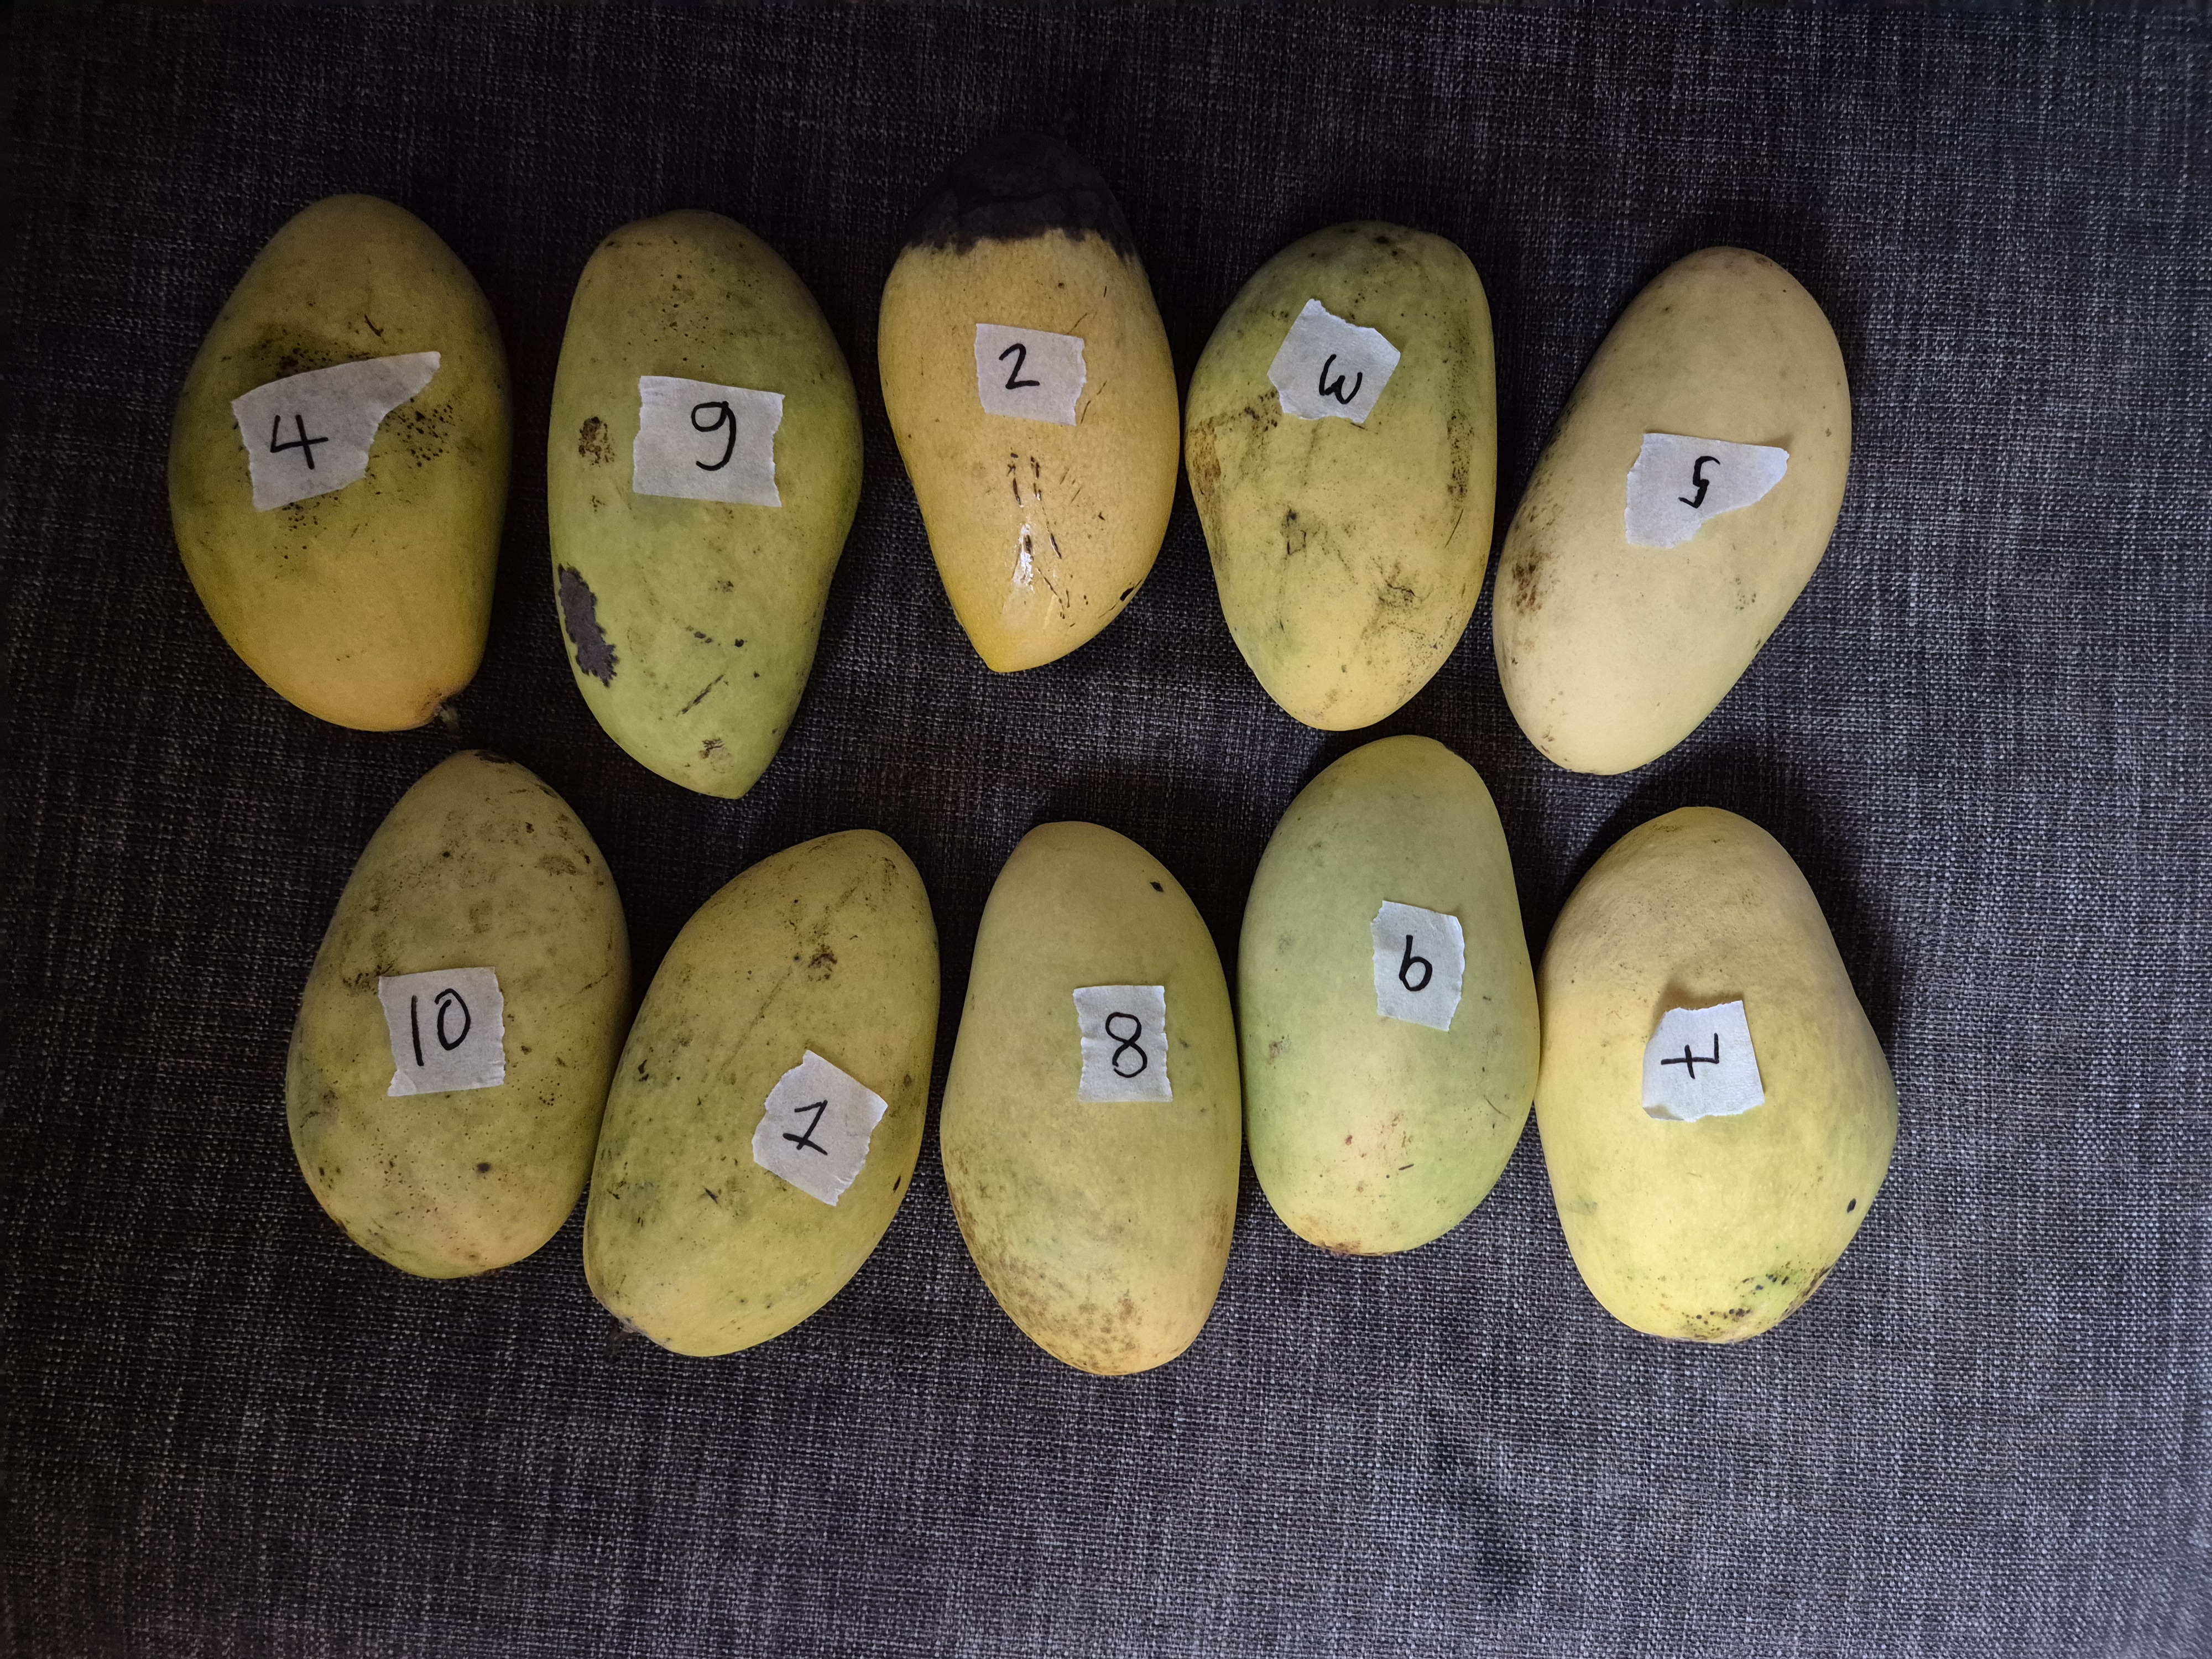
\includegraphics[width=0.45\textwidth]{/size-mango-test/ripe}
        \label{fig:ripe-mango}
    }
    \caption{Mangoes Tested for Size Measurement}
    \label{fig:mango_size_test}
\end{figure}

% todo explain the unripe and ripe mango imgs fig show above

\begin{figure}[!htbp]
	\centering
	\includegraphics[width=1\textwidth]{/size_new_graph/fig01}
	\caption{Length Comparison in cm}
	\label{fig:length_cm}
\end{figure}

% todo explain the length and width comparison in cm fig above and below

\begin{figure}[!htbp]
	\centering
	\includegraphics[width=1\textwidth]{/size_new_graph/fig02}
	\caption{Width Comparison in cm}
	\label{fig:width_cm}
\end{figure}

\begin{figure}[!htbp]
    \centering
    \subbottom[Absolute Difference for Length in cm]{
        \includegraphics[width=0.45\textwidth]{/size_new_graph/fig05}
        \label{fig:abs_length}
    }
    \hfill
    \subbottom[Absolute Difference for Width in cm]{
        \includegraphics[width=0.45\textwidth]{/size_new_graph/fig06}
        \label{fig:abs_width}
    }
    \vfill
    \subbottom[Percent Difference for Length]{
        \includegraphics[width=0.45\textwidth]{/size_new_graph/fig03}
        \label{fig:percent_diff_length}
    }
    \hfill
    \subbottom[Percent Difference for Width]{
        \includegraphics[width=0.45\textwidth]{/size_new_graph/fig04}
        \label{fig:percent_diff_width}
    }
    \caption{Percent and Absolute Difference between Both Methods}
    \label{fig:percent_absolute_diff}
\end{figure}

% todo will add explanation of the absolute and percent diff for the four graphs

\section{Formula with User Priority } \label{sec:userPriorityFormula}
% \gls{not:bprio} and \gls{not:rprio} and \gls{not:sprio} are the \gls{User Priority-Based Grading} for bruises, ripeness, and size of the Carabao mango. 
% Furthermore, \gls{not:bpred} and \gls{not:rpred} and \gls{not:spred} are the machine learning's predictions for bruises, ripeness, and size of the Carabao mango.
% The formula for the user priority is given by:
% \begin{equation}
% 	\label{eq:userPriority}	
%   \text{Mango Grade} = \ensuremath{b \left( P \right)  B\left( P \right) + r \left( P \right) R\left( P \right) + s \left( P \right) S\left( P \right)}
% \end{equation}
%
% \noindent The machine learning predictions are assigned the following numerical values shown below.
%
% \subsection{Ripeness Scores:}
% \begin{align}
% r(\text{yellow}) &= 1.0 \\
% r(\text{yellow\_green}) &= 2.0 \\
% r(\text{green}) &= 3.0
% \end{align}
%
% \subsection{Bruises Scores:}
% \begin{align}
% b(\text{bruised}) &= 1.0 \\
% b(\text{unbruised}) &= 2.0
% \end{align}
%
% \subsection{Size Scores:}
% \begin{align}
% s(\text{small}) &= 1.0 \\
% s(\text{medium}) &= 2.0 \\
% s(\text{large}) &= 3.0
% \end{align}
%

The Figures \ref{fig:bruises-only-input}, \ref{fig:ripeness-bruises-only-input} and 
\ref{fig:ripeness-only-input} are explained in this section where the inputted weight
values are all real number since negative and imaginary number are not allowed. The
purpose of this section is to demonstrate the different possible cases of using 
the zero value in the user priority.


\begin{figure}[!htbp]
	\centering
	\includegraphics[width=0.8\textwidth]{/priority/bruises-only}
	\caption{Only Bruises as a None Zero Value}
	\label{fig:bruises-only-input}
\end{figure}

An example of where the user only prioritizes bruises is shown on Figure~\ref{fig:bruises-only-input}.
This implies that the user disregards the ripeness and the size of the Carabao mangoes 
by setting the input priority value to zero.

\begin{figure}[!htbp]
	\centering
	\includegraphics[width=0.8\textwidth]{/priority/ripeness-and-bruises-only}
	\caption{Only Ripeness and Bruises as a None Zero Value}
	\label{fig:ripeness-bruises-only-input}
\end{figure}

Another example shown on Figure~\ref{fig:ripeness-bruises-only-input} shows where the user only
prioritized two mango charactgeristics which are the bruises and the ripeness. This is because 
the user set the size to zero. As such when grading the mangoes, it would still show the prediction
of the size however when grading the Carabao mango it would disregard the size in its calculation.

\begin{figure}[!htbp]
	\centering
	\includegraphics[width=0.8\textwidth]{/priority/ripeness-only}
	\caption{Only Ripeness as a None Zero Value}
	\label{fig:ripeness-only-input}
\end{figure}

Another similar user priority input to Figure~\ref{fig:bruises-only-input} is 
Figure~\ref{fig:ripeness-only-input} where it only prioritizes one parameter which is the ripeness.
Furthermore, notice the range of values for each grade has a maximum of 3.00 and a minimum of 1.00.
This is because the input weight of the ripeness is 1.0 meaning that the possible values are 1.00, 2.00, and 3.00.

\section{Physical Prototype} \label{sec:physicalPrototype}

For the physical prototype, there are two main parts which are the image acquisition system and
the conveyor belt. Both of these parts are being controllered by an \acr{RPi} through a python script.
For the first version of the prototype, Figure~\ref{fig:v1_prototype} shows three images which are 
the top view, entrance view of the Carabao mangoes and the side view of the prototype.
Notice that it is a barebone prototype made out of plywood with four rollers and black matte sheets.
to move the Carabao mangoes. There are two DC motors controlling each conveyor belt.
As seen on the side of the prototype on Figure~\ref{fig:v1_prototype}, the black sheet is not 
flexible and too stiff to be able to move it with the mangoes. This means that the conveyor 
belt would not be able to rotate and move the Carabao mangoes consistency.

\begin{figure}[!htbp]
    \centering
    \subbottom[Prototype Top View]{
        \includegraphics[width=0.45\textwidth]{top_view}
        \label{fig:top_view}
    }
    \hfill
    \subbottom[Entrance Conveyor Belt View]{
        \includegraphics[width=0.45\textwidth]{side1}
        \label{fig:side1}
    }
    \vfill
    \subbottom[Side Conveyor Belt View]{
        \includegraphics[width=0.45\textwidth]{side2}
        \label{fig:side2}
    }
    \caption{Version 1 of the Prototype}
    \label{fig:v1_prototype}
\end{figure}

% todo explain the shown electronics such as dc motors, relays breadboard, rpi etc

\begin{figure}[!htbp]
    \centering
    \subbottom[Prototype Main Hardware]{
        \includegraphics[width=0.45\textwidth]{schematic1}
        \label{fig:schematic1}
    }
    \hfill
    \subbottom[DC Motor and Pulley]{
        \includegraphics[width=0.45\textwidth]{DC_Motor_Pulley}
        \label{fig:dc_motor_pulley}
    }
    \vfill
    \subbottom[LED Lights and Camera Module]{
        \includegraphics[width=0.45\textwidth]{camera}
        \label{fig:camera}
    }
    \caption{Hardware View}
    \label{fig:hardware_view}
\end{figure}

% todo explain the improved prototype version 2 which are the conveyor belt and enclosing the 
% prototype on the same black sheet

\begin{figure}[!htbp]
    \centering
    \subbottom[Side View of Improved Prototype]{
        \includegraphics[width=0.45\textwidth]{new-side-view}
        \label{fig:new-side-view}
    }
    \hfill
    \subbottom[Top View of Improved Prototype]{
        \includegraphics[width=0.45\textwidth]{new-top-view}
        \label{fig:new-top-view}
    }
    \caption{Version 2: Improved Prototype}
    \label{fig:v2_prototype}
\end{figure}

\section{Software Application}

For the software application inside the \acr{RPi}, CustomTkinter is used as the main 
GUI for the python application. For the versions, there are two main versions. 
The first version which involves a fully automated capturing of both sides of the Carabao mango
and the second version which uses a part by part picturing and moving of mangoes. 
% todo explain the features of the intial prorotype and its problems
\begin{figure}[!htbp]
    \centering
    \subbottom[Version 1.1]{
        \includegraphics[width=0.45\textwidth]{UI_v1}
        \label{fig:ui_v1}
    }
    \hfill
    \subbottom[Version 1.2]{
        \includegraphics[width=0.45\textwidth]{UI_v2}
        \label{fig:ui_v2}
    }
    \vfill
    \subbottom[Version 1.3]{
        \includegraphics[width=0.45\textwidth]{UI_v3}
        \label{fig:ui_v3}
    }

    \caption{Version 1 of the RPi's User Interface}
    \label{fig:user_interface_v1}
\end{figure}

% todo explain the second version and its upgrades to the first version

\begin{figure}[!htbp]
    \centering
    \subbottom[Version 2.1 with Background Image]{
        \includegraphics[width=0.45\textwidth]{/ui/ui-version1}
        \label{fig:app_v4}
    }
    \hfill
    \subbottom[Version 2.2 without Background Image]{
        \includegraphics[width=0.45\textwidth]{/ui/ui-version2}
        \label{fig:app_v5}
    }
    \caption{Version 2 of the RPi's User Interface}
    \label{fig:ui_main_v2}
\end{figure}

% todo explain how it sorts the Carabao mango images

\begin{figure}[!htbp]
    \centering
    \subbottom[Version 1]{
        \includegraphics[width=0.45\textwidth]{sort_tree_1}
        \label{fig:sort_tree}
    }
    \hfill
    \subbottom[Version 2]{
        \includegraphics[width=0.45\textwidth]{sort_folder}
        \label{fig:sort_folder}
    }
    \vfill
    \subbottom[Version 3]{
        \includegraphics[width=0.45\textwidth]{sort_input_prior}
        \label{fig:input_folder_prior}
    }

    \caption{Mango Image Sorted}
    \label{fig:img_sorted}
\end{figure}

\begin{figure}[!htbp]
    \centering
    \subbottom[All Zero Error]{
        \includegraphics[width=0.45\textwidth]{/errors/all-zero}
        \label{fig:all-zero}
        \includegraphics[width=0.45\textwidth]{/errors/input-error}
    }
    \hfill
    \subbottom[Input Error]{
        \label{fig:input-error}
    }
    \vfill
    \subbottom[Null Button Error]{
        \includegraphics[width=0.45\textwidth]{/errors/null-button}
        \label{fig:null-button}
    }

    \caption{Error Messages}
    \label{fig:error-handel-1}
\end{figure}

\begin{figure}[!htbp]
    \centering
    \subbottom[Not Number at Conveyor Time]{
        \includegraphics[width=0.45\textwidth]{/errors/letter-time}
        \label{fig:letter-time}
    }
    \hfill
    \subbottom[Not Number at Priority]{
        \includegraphics[width=0.45\textwidth]{/errors/letter-priority}
        \label{fig:letter-priority}
    }
    \caption{Error message for Letter as Input}
    \label{fig:error-handel-2}
\end{figure}

\begin{figure}[!htbp]
	\centering
	\includegraphics[width=0.8\textwidth]{/ui/help}
	\caption{Help Page UI}
	\label{fig:help_page}
\end{figure}

\begin{figure}[!htbp]
    \centering
    \subbottom[Green and Unbruised]{
        \includegraphics[width=0.45\textwidth]{/ripe-class/green}
        \label{fig:green-result}
    }
    \hfill
    \subbottom[Yellow\_Green and Bruised]{
        \includegraphics[width=0.45\textwidth]{/ripe-class/yellow-green}
        \label{fig:yellow-green-result}
    }
    \vfill
    \subbottom[Yellow and Bruised]{
        \includegraphics[width=0.45\textwidth]{/ripe-class/yellow}
        \label{fig:yellow-result}
    }

    \caption{Sample Ripeness and Bruises Results}
    \label{fig:ripeness-all}
\end{figure}



% Table 1: CNN Training Results for GPU
\begin{table}[htbp]
\centering
\begin{tabular}{l|c|c|c|c|c|c}
\hline \hline
\textbf{Network} & \textbf{Prec} & \textbf{Rec} & \textbf{F1} & \textbf{Acc} & \textbf{Time} & \textbf{VRAM} \\
\hline
VGG16 & 0.188 & 0.434 & 0.263 & 43 & 2h57m & 7.0 \\
\hline
ALEXNET & 0.188 & 0.434 & 0.263 & 43 & 4h23m & 2.3 \\
\hline
RESNET50 & 0.870 & 0.869 & 0.868 & 87 & 7h13m & 4.1 \\
\hline
GOOGLENET & 0.898 & 0.895 & 0.892 & 89 & 3h3m & 2.9 \\
\hline
MOBILENETV2 & 0.898 & 0.898 & 0.897 & 90 & 2h0m & 3.6 \\
\hline
DENSENET121 & 0.877 & 0.877 & 0.875 & 88 & 2h10m & 5.5 \\
\hline
EFFICIENTNET B0 & 0.890 & 0.888 & 0.887 & 89 & 2h26m & 4.1 \\
\hline
EFFICIENTNET B1 & 0.867 & 0.862 & 0.859 & 86 & 2h30m & 5.3 \\
\hline
EFFICIENTNET B2 & 0.927 & 0.924 & 0.925 & 92 & 2h14m & 5.5 \\
\hline
EFFICIENTNET B3 & 0.882 & 0.880 & 0.879 & 88 & 2h25m & 6.8 \\
\hline
EFFICIENTNET B4 & 0.899 & 0.898 & 0.896 & 90 & 2h50m & 8.0 \\
\hline
EFFICIENTNET B5 & 0.925 & 0.924 & 0.924 & 92 & 5h49m & 11.6 \\
\hline
EFFICIENTNET B6 & 0.934 & 0.933 & 0.933 & 93 & 7h51m & 14.5 \\
\hline
EFFICIENTNET B7 & 0.883 & 0.871 & 0.873 & 87 & 10h34m & 18.8 \\
\hline
EFFICIENTNETV2-B0 & 0.915 & 0.913 & 0.913 & 91 & 1h53m & 3.0 \\
\hline
EFFICIENTNETV2-B1 & 0.904 & 0.904 & 0.902 & 90 & 2h0m & 3.6 \\
\hline
EFFICIENTNETV2-B2 & 0.902 & 0.900 & 0.901 & 90 & 2h17m & 3.8 \\
\hline
EFFICIENTNETV2-B3 & 0.926 & 0.926 & 0.925 & 93 & 2h2m & 4.5 \\
\hline
EFFICIENTNETV2-S & 0.894 & 0.893 & 0.891 & 89 & 1h59m & 6.1 \\
\hline
EFFICIENTNETV2-M & 0.893 & 0.893 & 0.892 & 89 & 2h58m & 9.9 \\
\hline
EFFICIENTNETV2-L & 0.875 & 0.871 & 0.870 & 87 & 14h58m & 16.8 \\
\hline
\textbf{AVERAGE} & \textbf{0.830} & \textbf{0.852} & \textbf{0.835} & \textbf{85} & \textbf{--} & \textbf{7.0} \\
\hline
\end{tabular}
\caption{More CNN Training Results for GPU}
\label{tab:more_cnn_training_gpu}
\end{table}

% Table 2: CNN Training Results for CPU
\begin{table}[htbp]
\centering
\begin{tabular}{l|c|c|c|c|c|c}
\hline \hline
\textbf{Network} & \textbf{Prec} & \textbf{Rec} & \textbf{F1} & \textbf{Acc} & \textbf{Time} & \textbf{Mem} \\
\hline
VGG16 & 0.297 & 0.545 & 0.384 & 54 & 5h38m & 6.5 \\
\hline
ALEXNET & 0.297 & 0.545 & 0.384 & 54 & 4h25m & 3.3 \\
\hline
RESNET50 & 0.858 & 0.844 & 0.844 & 84 & 8h24m & 5.4 \\
\hline
GOOGLENET & 0.843 & 0.808 & 0.799 & 81 & 3h14m & 4.0 \\
\hline
MOBILENETV2 & 0.859 & 0.858 & 0.858 & 86 & 3h44m & 4.8 \\
\hline
DENSENET121 & 0.839 & 0.838 & 0.838 & 84 & 3h8m & 6.7 \\
\hline
EFFICIENTNET B0 & 0.873 & 0.870 & 0.870 & 87 & 2h37m & 5.3 \\
\hline
EFFICIENTNET B1 & 0.898 & 0.897 & 0.896 & 90 & 3h8m & 6.7 \\
\hline
EFFICIENTNET B2 & 0.901 & 0.901 & 0.901 & 90 & 2h56m & 6.7 \\
\hline
EFFICIENTNET B3 & 0.913 & 0.913 & 0.913 & 91 & 3h27m & 8.0 \\
\hline
EFFICIENTNET B4 & 0.897 & 0.897 & 0.897 & 90 & 4h17m & 9.8 \\
\hline
EFFICIENTNET B5 & 0.892 & 0.883 & 0.881 & 88 & 5h45m & 12.2 \\
\hline
EFFICIENTNET B6 & 0.884 & 0.883 & 0.882 & 88 & 7h12m & 14.5 \\
\hline
EFFICIENTNET B7 & 0.857 & 0.856 & 0.856 & 86 & 9h9m & 18.0 \\
\hline
EFFICIENTNETV2-B0 & 0.873 & 0.860 & 0.858 & 86 & 2h6m & 4.4 \\
\hline
EFFICIENTNETV2-B1 & 0.893 & 0.893 & 0.893 & 89 & 3h30m & 5.1 \\
\hline
EFFICIENTNETV2-B2 & 0.888 & 0.881 & 0.881 & 88 & 2h45m & 5.4 \\
\hline
EFFICIENTNETV2-B3 & 0.905 & 0.905 & 0.905 & 90 & 2h32m & 6.2 \\
\hline
EFFICIENTNETV2-S & 0.860 & 0.836 & 0.831 & 84 & 2h55m & 7.7 \\
\hline
EFFICIENTNETV2-M & 0.856 & 0.846 & 0.846 & 85 & 2h37m & 9.3 \\
\hline
EFFICIENTNETV2-L & 0.849 & 0.836 & 0.836 & 84 & 13h39m & 17.9 \\
\hline
\textbf{AVERAGE} & \textbf{0.820} & \textbf{0.838} & \textbf{0.821} & \textbf{84} & \textbf{--} & \textbf{8.0} \\
\hline

\end{tabular}
\caption{More CNN Training Results for CPU}
\label{tab:more_cnn_training_cpu}
\end{table}

% Table 3: Mango Size Results
\begin{table}[htbp]
\centering
\begin{tabular}{c|c|c|c|c|c|c|c}
\hline \hline
\multirow{2}{*}{\textbf{ID}} & \multirow{2}{*}{\textbf{Weight (g)}} & \multicolumn{2}{c|}{\textbf{Ground Truth}} & \multicolumn{2}{c|}{\textbf{V2 Code}} & \multicolumn{2}{c}{\textbf{V1 Code}} \\
\cline{3-8}
& & \textbf{L} & \textbf{W} & \textbf{L} & \textbf{W} & \textbf{L} & \textbf{W} \\
\hline
01 & 260.8 & 11.8 & 7.80 & 12.86 & 7.96 & 10.33 & 3.08 \\
\hline
02 & 299.4 & 12.8 & 7.80 & 14.69 & 8.30 & 11.59 & 3.73 \\
\hline
03 & 238.4 & 11.4 & 7.60 & 12.42 & 7.60 & 9.17 & 2.36 \\
\hline
04 & 335.6 & 13.8 & 10.50 & 15.38 & 9.33 & 12.49 & 5.00 \\
\hline
05 & 272.4 & 12.9 & 8.50 & 15.13 & 7.81 & 11.52 & 3.96 \\
\hline
06 & 267.9 & 13.1 & 8.20 & 15.72 & 7.73 & 11.78 & 3.58 \\
\hline
07 & 274.0 & 12.6 & 8.20 & 14.96 & 7.88 & 11.80 & 4.00 \\
\hline
08 & 272.3 & 13.3 & 8.00 & 15.56 & 7.49 & 12.02 & 4.26 \\
\hline
09 & 281.6 & 13.0 & 8.00 & 15.20 & 7.55 & 12.12 & 4.26 \\
\hline
10 & 286.2 & 13.8 & 8.00 & 15.20 & 7.55 & 12.17 & 3.09 \\
\hline
11 & 284.6 & 12.6 & 9.00 & 15.20 & 7.55 & 10.90 & 3.26 \\
\hline
12 & 265.7 & 13.3 & 8.00 & 14.80 & 8.48 & 11.38 & 2.98 \\
\hline
13 & 278.1 & 13.0 & 7.60 & 15.08 & 7.87 & 11.00 & 3.18 \\
\hline
14 & 263.8 & 12.9 & 7.50 & 15.11 & 7.75 & 11.28 & 4.11 \\
\hline
15 & 222.0 & 12.1 & 7.80 & 12.96 & 7.44 & 10.73 & 3.17 \\
\hline
16 & 240.1 & 13.5 & 8.20 & 15.36 & 7.14 & 11.15 & 3.21 \\
\hline
17 & 290.7 & 13.5 & 8.50 & 14.71 & 8.20 & 11.76 & 3.21 \\
\hline
18 & 260.1 & 12.8 & 8.00 & 14.52 & 7.65 & 10.91 & 3.12 \\
\hline
19 & 253.6 & 12.9 & 7.50 & 14.08 & 7.66 & 11.65 & 3.17 \\
\hline
20 & 225.9 & 12.0 & 7.50 & 13.17 & 7.48 & 10.49 & 3.24 \\
\hline
\textbf{AVG} & \textbf{264.1} & \textbf{12.8} & \textbf{8.1} & \textbf{14.7} & \textbf{7.8} & \textbf{11.3} & \textbf{3.5} \\
\hline

\end{tabular}
\caption{Mango Size Results}
\label{tab:more_size_results01}
\end{table}

% Table 4: Mango Size Difference to Ground Truth Results
\begin{table}[htbp]
\centering
\begin{tabular}{c|c|c|c|c}
\hline \hline
\multirow{2}{*}{\textbf{ID}} & \multicolumn{2}{c|}{\textbf{V2 Difference}} & \multicolumn{2}{c}{\textbf{V1 Difference}} \\
\cline{2-5}
& \textbf{L} & \textbf{W} & \textbf{L} & \textbf{W} \\
\hline
01 & 1.06 & 0.16 & 1.47 & 4.72 \\
\hline
02 & 1.89 & 0.50 & 1.21 & 4.07 \\
\hline
03 & 1.02 & 0.00 & 2.23 & 5.24 \\
\hline
04 & 1.58 & 1.17 & 1.31 & 5.50 \\
\hline
05 & 2.23 & 0.69 & 1.38 & 4.54 \\
\hline
06 & 2.62 & 0.47 & 1.32 & 4.62 \\
\hline
07 & 2.36 & 0.32 & 0.80 & 4.20 \\
\hline
08 & 2.26 & 0.51 & 1.28 & 3.74 \\
\hline
09 & 2.20 & 0.45 & 1.12 & 3.74 \\
\hline
10 & 1.40 & 0.45 & 1.63 & 4.91 \\
\hline
11 & 2.60 & 1.45 & 1.70 & 5.74 \\
\hline
12 & 1.50 & 0.48 & 1.92 & 5.02 \\
\hline
13 & 2.08 & 0.27 & 2.00 & 4.42 \\
\hline
14 & 2.21 & 0.25 & 1.62 & 3.39 \\
\hline
15 & 0.86 & 0.36 & 1.37 & 4.63 \\
\hline
16 & 1.86 & 1.06 & 2.35 & 4.99 \\
\hline
17 & 1.21 & 0.30 & 1.74 & 5.29 \\
\hline
18 & 1.72 & 0.35 & 1.89 & 4.88 \\
\hline
19 & 1.18 & 0.16 & 1.25 & 4.33 \\
\hline
20 & 1.17 & 0.02 & 1.51 & 4.26 \\
\hline
\textbf{AVG} & \textbf{1.80} & \textbf{0.50} & \textbf{1.60} & \textbf{4.60} \\
\hline

\end{tabular}
\caption{Mango Size Difference to Ground Truth Results}
\label{tab:more_size_results02}
\end{table}

% Table 5: Mean and Standard Deviation of Size
\begin{table}[htbp]
\centering
\begin{tabular}{l|c|c|c|c}
\hline \hline
\multirow{2}{*}{\textbf{Metric}} & \multicolumn{2}{c|}{\textbf{V2 Code}} & \multicolumn{2}{c}{\textbf{V1 Code}} \\
\cline{2-5}
& \textbf{Mean} & \textbf{SD} & \textbf{Mean} & \textbf{SD} \\
\hline
Length Differences (cm) & 1.75 & 0.56 & 1.54 & 0.40 \\
\hline
Width Differences (cm) & 0.47 & 0.37 & 4.61 & 0.61 \\
\hline
Length Percent Difference & 13.57\% & 4.20\% & 12.04\% & 3.28\% \\
\hline
Width Percent Difference & 3.24\% & 6.16\% & 56.89\% & 6.32\% \\
\hline

\end{tabular}
\caption{Mean and Standard Deviation of Size}
\label{tab:mean_and_std_results}
\end{table}

\section{Summary} \label{sec:summary_results_and_discussions}

Provide the gist of this chapter such that it reflects the contents and the message. This is a compile test
\\

